\subsection{Quality Attributes recommendations}

\mdavid{Expand on the explanation based on the diagram}
Figure \ref{fig:rslifecycle} is taken from the sub group 1 report \cite{sg1tf2023}

\begin{figure}[h]
    \centering
    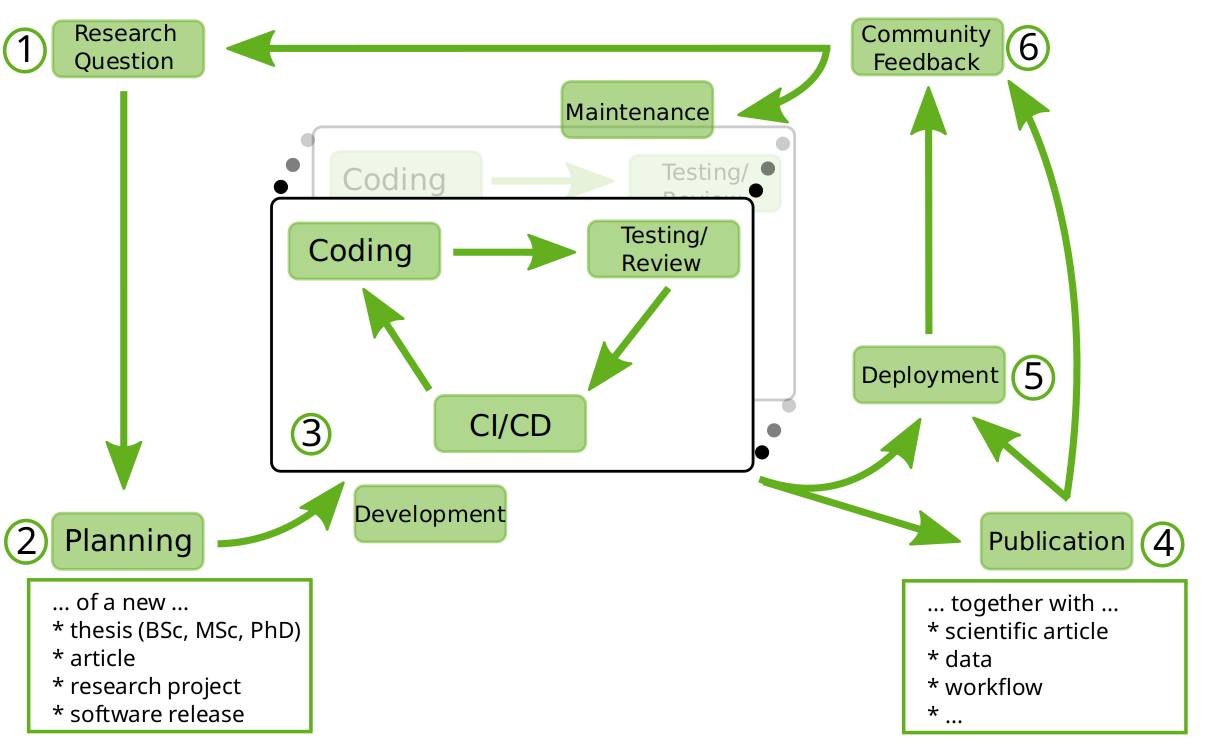
\includegraphics[width=0.99\linewidth]{imgs/rs_lifecycle.png}
    \caption{Research Software lifecycle.}
    \label{fig:rslifecycle}
\end{figure}



\subsubsection{User story: Individual development}

RS stack 4: \textbf{Project specific code} \newline
RS type 1: \textbf{Library}

\begin{itemize}
    \item \textbf{EOSC-SCMet-02}: \% of redundant code
    \item \textbf{EOSC-SCMet-10}: Number of comments
    \item \textbf{EOSC-Qual-27}: Intellectual Property
    \item \textbf{EOSC-SWRelMan-01}: Open source
    \item \textbf{EOSC-SWRelMan-02}: Version Control System (VCS)
    \item \textbf{EOSC-SWRelMan-10}: Open-source license
    \item \textbf{EOSC-SWRelMan-12}: Packaging
    \item \textbf{EOSC-SWRelMan-15}: Code deployment
    \item \textbf{EOSC-SWRelMan-29}: Documentation online
    \item \textbf{EOSC-SWRelMan-30}: Documentation updates
    \item \textbf{EOSC-SWTest-15}: No world-writable files or directories
\end{itemize}
\hrule

RS stack 4: \textbf{Project specific code} \newline
RS type 4: \textbf{Analysis script and workflows}

\begin{itemize}
    \item \textbf{EOSC-SCMet-02}: \% of redundant code
    \item \textbf{EOSC-SCMet-10}: Number of comments
    \item \textbf{EOSC-Qual-27}: Intellectual Property
    \item \textbf{EOSC-SWRelMan-01}: Open source
    \item \textbf{EOSC-SWRelMan-02}: Version Control System (VCS)
    \item \textbf{EOSC-SWRelMan-10}: Open-source license
    \item \textbf{EOSC-SWRelMan-29}: Documentation online
    \item \textbf{EOSC-SWRelMan-30}: Documentation updates
    \item \textbf{EOSC-SWTest-15}: No world-writable files or directories
\end{itemize}
\hrule

\subsubsection{User story: Team Project}

RS stack 4: \textbf{Project specific code} \newline
RS type 1: \textbf{Library}

\begin{itemize}
    \item \textbf{EOSC-SCMet-02}: \% of redundant code
    \item \textbf{EOSC-SCMet-10}: Number of comments
    \item \textbf{EOSC-TMet-02}: \# Resolved bugs
    \item \textbf{EOSC-TMet-03}: \# Open bugs
    \item \textbf{EOSC-Qual-27}: Intellectual Property
    \item \textbf{EOSC-SWRelMan-01}: Open source
    \item \textbf{EOSC-SWRelMan-02}: Version Control System (VCS)
    \item \textbf{EOSC-SWRelMan-03}: Source code hosting
    \item \textbf{EOSC-SWRelMan-04}: Working state version
    \item \textbf{EOSC-SWRelMan-07}: Support
    \item \textbf{EOSC-SWRelMan-10}: Open-source license
    \item \textbf{EOSC-SWRelMan-12}: Packaging
    \item \textbf{EOSC-SWRelMan-15}: Code deployment
    \item \textbf{EOSC-SWRelMan-29}: Documentation online
    \item \textbf{EOSC-SWRelMan-30}: Documentation updates
    \item \textbf{EOSC-SWRelMan-32}: Documentation production
    \item \textbf{EOSC-SWTest-01}: Code style
    \item \textbf{EOSC-SWTest-02}: Unit tests
    \item \textbf{EOSC-SWTest-03}: Test doubles
    \item \textbf{EOSC-SWTest-07}: Functional testing
    \item \textbf{EOSC-SWTest-15}: No world-writable files or directories
\end{itemize}
\hrule

RS stack 4: \textbf{Project specific code} \newline
RS type 4: \textbf{Analysis script and workflows}

\begin{itemize}
    \item \textbf{EOSC-SCMet-02}: \% of redundant code
    \item \textbf{EOSC-SCMet-10}: Number of comments
    \item \textbf{EOSC-TMet-02}: \# Resolved bugs
    \item \textbf{EOSC-TMet-03}: \# Open bugs
    \item \textbf{EOSC-Qual-27}: Intellectual Property
    \item \textbf{EOSC-SWRelMan-01}: Open source
    \item \textbf{EOSC-SWRelMan-02}: Version Control System (VCS)
    \item \textbf{EOSC-SWRelMan-03}: Source code hosting
    \item \textbf{EOSC-SWRelMan-04}: Working state version
    \item \textbf{EOSC-SWRelMan-07}: Support
    \item \textbf{EOSC-SWRelMan-10}: Open-source license
    \item \textbf{EOSC-SWRelMan-29}: Documentation online
    \item \textbf{EOSC-SWRelMan-30}: Documentation updates
    \item \textbf{EOSC-SWTest-15}: No world-writable files or directories
\end{itemize}
\hrule

RS stack 4: \textbf{Project specific code} \newline
RS type 5: \textbf{Services and platforms}

\begin{itemize}
    \item \textbf{EOSC-SCMet-02}: \% of redundant code
    \item \textbf{EOSC-SCMet-10}: Number of comments
    \item \textbf{EOSC-TMet-02}: \# Resolved bugs
    \item \textbf{EOSC-TMet-03}: \# Open bugs
    \item \textbf{EOSC-Qual-27}: Intellectual Property
    \item \textbf{EOSC-SWRelMan-01}: Open source
    \item \textbf{EOSC-SWRelMan-02}: Version Control System (VCS)
    \item \textbf{EOSC-SWRelMan-03}: Source code hosting
    \item \textbf{EOSC-SWRelMan-04}: Working state version
    \item \textbf{EOSC-SWRelMan-07}: Support
    \item \textbf{EOSC-SWRelMan-10}: Open-source license
    \item \textbf{EOSC-SWRelMan-12}: Packaging
    \item \textbf{EOSC-SWRelMan-15}: Code deployment
    \item \textbf{EOSC-SWRelMan-29}: Documentation online
    \item \textbf{EOSC-SWRelMan-30}: Documentation updates
    \item \textbf{EOSC-SWRelMan-32}: Documentation production
    \item \textbf{EOSC-SWTest-01}: Code style
    \item \textbf{EOSC-SWTest-02}: Unit tests
    \item \textbf{EOSC-SWTest-03}: Test doubles
    \item \textbf{EOSC-SWTest-05}: API testing
    \item \textbf{EOSC-SWTest-06}: Integration testing
    \item \textbf{EOSC-SWTest-15}: No world-writable files or directories
    \item \textbf{EOSC-SWTest-16}: Public endpoints and APIs encrypted
    \item \textbf{EOSC-SWTest-17}: Strong ciphers
    \item \textbf{EOSC-SWTest-18}: Authentication and Authorization
    \item \textbf{EOSC-SWTest-20}: Service compliance with data regulations (GDPR)
\end{itemize}
\hrule

\subsubsection{User story: Team OSS}

RS stack 3 and 2: \textbf{Domain specific tools} and  \textbf{Scientific infrastructure} \newline
RS type 1: \textbf{Library}

\begin{itemize}
    \item \textbf{EOSC-SCMet-02}: \% of redundant code
    \item \textbf{EOSC-SCMet-10}: Number of comments
    \item \textbf{EOSC-TMet-02}: \# Resolved bugs
    \item \textbf{EOSC-TMet-03}: \# Open bugs
    \item \textbf{EOSC-TMet-04}: Defect rates
    \item \textbf{EOSC-Qual-27}: Intellectual Property
    \item \textbf{EOSC-SWRelMan-01}: Open source
    \item \textbf{EOSC-SWRelMan-02}: Version Control System (VCS)
    \item \textbf{EOSC-SWRelMan-03}: Source code hosting
    \item \textbf{EOSC-SWRelMan-04}: Working state version
    \item \textbf{EOSC-SWRelMan-07}: Support
    \item \textbf{EOSC-SWRelMan-08}: Code review
    \item \textbf{EOSC-SWRelMan-10}: Open-source license
    \item \textbf{EOSC-SWRelMan-12}: Packaging
    \item \textbf{EOSC-SWRelMan-15}: Code deployment
    \item \textbf{EOSC-SWRelMan-26}: Documentation version controlled
    \item \textbf{EOSC-SWRelMan-27}: Documentation as code
    \item \textbf{EOSC-SWRelMan-28}: Documentation formats
    \item \textbf{EOSC-SWRelMan-29}: Documentation online
    \item \textbf{EOSC-SWRelMan-30}: Documentation updates
    \item \textbf{EOSC-SWRelMan-32}: Documentation production
    \item \textbf{EOSC-SWTest-01}: Code style
    \item \textbf{EOSC-SWTest-02}: Unit tests
    \item \textbf{EOSC-SWTest-03}: Test doubles
    \item \textbf{EOSC-SWTest-07}: Functional testing
    \item \textbf{EOSC-SWTest-08}: Performance testing
    \item \textbf{EOSC-SWTest-13}: Static Application Security Testing (SAST)
    \item \textbf{EOSC-SWTest-14}: Security code reviews
    \item \textbf{EOSC-SWTest-15}: No world-writable files or directories
\end{itemize}
\hrule

RS stack 3 and 2: \textbf{Domain specific tools} and \textbf{Scientific infrastructure} \newline
RS type 2 and 3: \textbf{Framework, Application}

\begin{itemize}
    \item \textbf{EOSC-SCMet-02}: \% of redundant code
    \item \textbf{EOSC-SCMet-10}: Number of comments
    \item \textbf{EOSC-TMet-02}: \# Resolved bugs
    \item \textbf{EOSC-TMet-03}: \# Open bugs
    \item \textbf{EOSC-TMet-04}: Defect rates
    \item \textbf{EOSC-Qual-27}: Intellectual Property
    \item \textbf{EOSC-SWRelMan-01}: Open source
    \item \textbf{EOSC-SWRelMan-02}: Version Control System (VCS)
    \item \textbf{EOSC-SWRelMan-03}: Source code hosting
    \item \textbf{EOSC-SWRelMan-04}: Working state version
    \item \textbf{EOSC-SWRelMan-07}: Support
    \item \textbf{EOSC-SWRelMan-08}: Code review
    \item \textbf{EOSC-SWRelMan-10}: Open-source license
    \item \textbf{EOSC-SWRelMan-12}: Packaging
    \item \textbf{EOSC-SWRelMan-15}: Code deployment
    \item \textbf{EOSC-SWRelMan-26}: Documentation version controlled
    \item \textbf{EOSC-SWRelMan-27}: Documentation as code
    \item \textbf{EOSC-SWRelMan-28}: Documentation formats
    \item \textbf{EOSC-SWRelMan-29}: Documentation online
    \item \textbf{EOSC-SWRelMan-30}: Documentation updates
    \item \textbf{EOSC-SWRelMan-32}: Documentation production
    \item \textbf{EOSC-SWTest-01}: Code style
    \item \textbf{EOSC-SWTest-02}: Unit tests
    \item \textbf{EOSC-SWTest-03}: Test doubles
    \item \textbf{EOSC-SWTest-04}: Test-Driven Development (TDD)
    \item \textbf{EOSC-SWTest-07}: Functional testing
    \item \textbf{EOSC-SWTest-08}: Performance testing
    \item \textbf{EOSC-SWTest-10}: Scalability testing
    \item \textbf{EOSC-SWTest-13}: Static Application Security Testing (SAST)
    \item \textbf{EOSC-SWTest-14}: Security code reviews
    \item \textbf{EOSC-SWTest-15}: No world-writable files or directories
\end{itemize}
\hrule

\subsubsection{User story: Team Service}

RS stack 3 and 2: \textbf{Domain specific tools} and \textbf{Scientific infrastructure} \newline
RS type 5: \textbf{Services and platforms}

\begin{itemize}
    \item \textbf{EOSC-SCMet-02}: \% of redundant code
    \item \textbf{EOSC-SCMet-10}: Number of comments
    \item \textbf{EOSC-TMet-02}: \# Resolved bugs
    \item \textbf{EOSC-TMet-03}: \# Open bugs
    \item \textbf{EOSC-TMet-04}: Defect rates
    \item \textbf{EOSC-Qual-27}: Intellectual Property
    \item \textbf{EOSC-SWRelMan-01}: Open source
    \item \textbf{EOSC-SWRelMan-02}: Version Control System (VCS)
    \item \textbf{EOSC-SWRelMan-03}: Source code hosting
    \item \textbf{EOSC-SWRelMan-04}: Working state version
    \item \textbf{EOSC-SWRelMan-07}: Support
    \item \textbf{EOSC-SWRelMan-08}: Code review
    \item \textbf{EOSC-SWRelMan-10}: Open-source license
    \item \textbf{EOSC-SWRelMan-12}: Packaging
    \item \textbf{EOSC-SWRelMan-15}: Code deployment
    \item \textbf{EOSC-SWRelMan-26}: Documentation version controlled
    \item \textbf{EOSC-SWRelMan-27}: Documentation as code
    \item \textbf{EOSC-SWRelMan-28}: Documentation formats
    \item \textbf{EOSC-SWRelMan-29}: Documentation online
    \item \textbf{EOSC-SWRelMan-30}: Documentation updates
    \item \textbf{EOSC-SWRelMan-32}: Documentation production
    \item \textbf{EOSC-SWTest-01}: Code style
    \item \textbf{EOSC-SWTest-02}: Unit tests
    \item \textbf{EOSC-SWTest-03}: Test doubles
    \item \textbf{EOSC-SWTest-04}: Test-Driven Development (TDD)
    \item \textbf{EOSC-SWTest-05}: API testing
    \item \textbf{EOSC-SWTest-06}: Integration testing
    \item \textbf{EOSC-SWTest-08}: Performance testing
    \item \textbf{EOSC-SWTest-09}: Stress testing
    \item \textbf{EOSC-SWTest-10}: Scalability testing
    \item \textbf{EOSC-SWTest-12}: Open Web Application Security Project (OWASP)
    \item \textbf{EOSC-SWTest-13}: Static Application Security Testing (SAST)
    \item \textbf{EOSC-SWTest-14}: Security code reviews
    \item \textbf{EOSC-SWTest-15}: No world-writable files or directories
    \item \textbf{EOSC-SWTest-16}: Public endpoints and APIs encrypted
    \item \textbf{EOSC-SWTest-17}: Strong ciphers
    \item \textbf{EOSC-SWTest-18}: Authentication and Authorization
    \item \textbf{EOSC-SWTest-19}: API security assessment
    \item \textbf{EOSC-SWTest-20}: Service compliance with data regulations (GDPR)
    \item \textbf{EOSC-SWTest-21}: Dynamic Application Security Testing (DAST)
    \item \textbf{EOSC-SWTest-22}: Interactive Application Security Testing (IAST)
    \item \textbf{EOSC-SWTest-23}: Security penetration testing
    \item \textbf{EOSC-SWTest-24}: Security assessment
    \item \textbf{EOSC-SWTest-25}: Security as Code (SaC) Testing
\end{itemize}
\hrule

\subsection{Example of tools, services and infrastructures to implement Quality Assurance for RS}

% \violaine{The idea is to refer to some search software of the different categories and show the similarities and differences with
% the analysis of the top to point out the possible lacks in the current service offer} 
